
\section{Introduction}
A recent trend in the 3D face reconstruction research has been to emboss fine high-frequency details to the reconstruction with methods like shape-from-shading \cite{or2015rgbd} or mesoscopic augmentations \cite{beeler2010high}. While not always reflecting the true geometry of the surface, these methods add realism to the mesh, which can be desirable for purposes like animation. Such methods can easily be applied to our reconstructions as well. We modify the mesoscopic augmentation method proposed in \cite{sela2017unrestricted} so that the underlying geometry is preserved, and apply it to our meshes. Since these are based on a dark-is-deep assumption, we skip quantitative evaluation, and provide qualitative results in Fig.\ref{fig:high_freq}. Details on the modified approach are provided in the supplementary.

 \begin{figure}
\begin{center}
  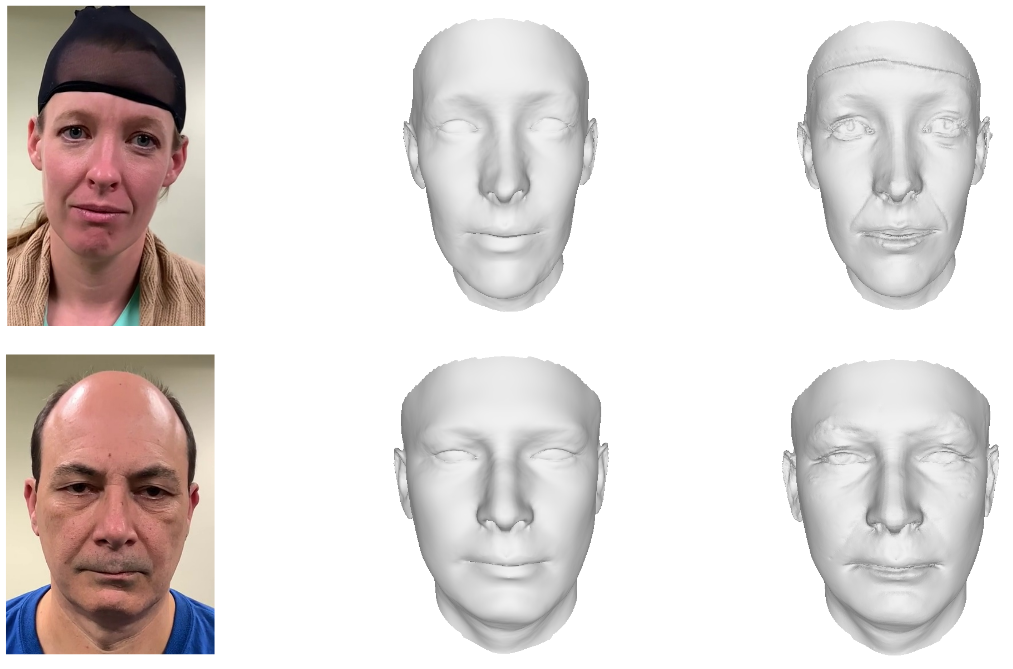
\includegraphics[width=0.8\linewidth]{images/meso_new.png}
\end{center}
  \caption{(Centre) Ours. (Right) Ours with modified mesoscopic augmentations.}
\label{fig:high_freq}
\end{figure}
Recently, Sela \etal\cite{sela2017unrestricted} showed impressive results by interpreting the idea of high frequency mesoscopic augmentations \cite{beeler2010high} through mesh heat flows. In our experiments, we found this method to not adapt well to ``in-the-wild" images, distorting the mesh too much due to sensor noise/unconstrained lighting. We make some modifications to their method to add details without losing the underlying mesh structure.\\
Since this method is based on a "dark-is-deep" assumption and not necessarily founded in geometry, we skip quantitative evaluation for these results and simply provide qualitative comparisons between our reconstructions, with and without our augmentation scheme, compared to the augmentation scheme of \cite{sela2017unrestricted}.

\section{Our Approach}

Beeler \etal \cite{beeler2010high} proposed using a high-pass filtered version of the texture to emboss a mesh with fine details, such as wrinkled and pores. The recent work of Sela \etal \cite{sela2017unrestricted} proposed using the mesh itself to obtain the high frequency component of the texture, using heat flow to model a low pass filterer version of the texture. In their results, this modification allows them to capture more medium-to-fine scale details, such as the nasolabial folds. However, we observed that their method also tends to distort the mesh, and also pick up on other high frequency noise such as sensor noise that is not desirable. We thus propose to augment our reconstructions as follows: \\
For a mesh with per vertex texture mapping $\tau_{v}$, we calculate a low-pass filtered version of the texture as :
\begin{align}
\tau_{lp} = (M-dt.C)^{-1}.M\tau_{v}
 \label{eqn:mesoscopic}
\end{align}
Where M and C are the mesh mass matrix and cotangent Laplacian matrix. dt is set to a small constant value of $0.001$. This has the effect of removing noisy effects like sensor noise from $\tau_{lp}$

We then calculate a band-pass version of the texture, where we wish to capture the medium-high frequency details in the texture:
\begin{align}
\mu_{v} = \tau_{lp} - (M-\Delta t.C)^{-1}.M\tau_{v}
 \label{eqn:mesoscopic}
\end{align}
Where $\Delta t = 0.01$. \\
Now, $\mu_{v}$ ,the band-pass version of the texture map is used to calculate the per vertex deformation, such that vertices which deviate more from the mean of the band pass texture are deformed more :
\begin{align}
\vec{\delta_{\mu}}(v)= || \mu_{v}(v) - \mu_{m} ||.\vec{n}(v)
\end{align}
Where $\mu_{m}$ is the mean of $\mu_{v}$, and $\vec{n}(v)$ is the normal vector of vertex v.
% \begin{align}
% \delta_{\mu}(v)=\frac{\underset{v_{i}\in\mathcal{N}(v)}{\sum}\alpha_{(v,v_{i})}\left(\mu(v)-\mu(v_{i})\right)\left(1-\frac{\left|\langle v-v_{i},\vec{n}(v)\rangle\right|}{\|v-v_{i}\|}\right)}{\underset{v_{i}\in\mathcal{N}(v)}{\sum}\alpha_{(v,v_{i})}},
%  \label{eqn:mesoscopic}
% \end{align}
% where $\alpha_{(v,v_i)} = \exp{\left(-\|v-v_i\|\right)}$.

Although this per vertex deformation can be applied to the mesh directly, for "smoother" results, it can be plugged into the mesh fitting optimization as described in Sec 3.3.4 , so that the mesh fitting energy becomes: 

 $$ \arg \min_{V}  E_{pcl} + \alpha E_{lms} + \beta E_{edges} +  \gamma E_{reg} + \lambda E_{meso} $$
 Where $E_{meso}$ is the distance between the current vertex location and the desired location calculated using $\delta_{\mu}(v)$

This simplified version of the original approach suggested by \cite{beeler2010high} allows us to capture details like eye-lids, lip corners and nasolabial-folds in the mesh.


